\documentclass[11pt, titlepage]{article}

\usepackage[margin=1in]{geometry}
\usepackage[strict]{changepage}
\usepackage{float}
\usepackage{fancyhdr}
\usepackage{mhchem}
\usepackage{siunitx}
\usepackage{wrapfig, booktabs}
\usepackage{enumitem}
\usepackage{caption}
\usepackage{commath}
\usepackage{amsmath}
\usepackage[hang]{footmisc}
\usepackage{multicol}
\usepackage{amsfonts}
\usepackage{mathrsfs}
\usepackage{mathtools}
\usepackage{tikz}

% my imports
\usepackage[most]{tcolorbox}
\usepackage{hyperref}
\hypersetup{
    colorlinks,
    citecolor=black,
    filecolor=black,
    linkcolor=black,
    urlcolor=black
}

\newcommand{\experimentDate}{\today}
\newcommand{\className}{CSE 371}
\newcommand{\assignmentname}{Lab 2}
\author{Cameron Jennings (ID: 2029631), Donovan Clay (ID: 2276005)}
\newcommand{\authorLastName}{Jennings, Clay}
\title{\assignmentname}

\date{\parbox{\linewidth}{\centering
\experimentDate
  \endgraf\bigskip
  \className\
}}

\pagestyle{fancy}
\fancyhf{}
\setlength{\headheight}{13.59999pt}
\rhead{\authorLastName\ \thepage}
% \lhead{\experimentShortName}
\lhead{\hyperref[beginning]{\assignmentname}}
\cfoot{\className\ -- \assignmentname}

\usepackage{color}
\usepackage{sectsty}

\definecolor{WordSectionBlue}{RGB}{30, 90, 147}

\allsectionsfont{\color{WordSectionBlue}}

\tcbuselibrary{breakable}


\begin{document}
	\maketitle
 
    \setcounter{tocdepth}{2}
    \begin{center}
        \tableofcontents\label{beginning}
    \end{center}
    \newpage
    
    \section{Design Procedure}
    In this lab, we were tasked to implement computer memory or RAM. The memory module is to have 32 addresses and 3 bits per address to store data. The inputs of the RAM are a signal to determine if we are reading or writing a value, data to fill the bits in an address when the system is notified to write, and an address to determine what address we are reading or writing. Additionally, the system uses switches and HEX displays of the DE1\_SoC board to process data. The switches control the address, data, and write signal being input to the system, while the HEX displays output what address(es) is being used and the number within that address. \\

    In total, there were three different tasks to complete. Tasks 1 and 3 consisted of using modules defined in the Quartus library to run our system. Task 2 was to be implemented using SystemVerilog on our own. \\
    
        \subsection{Task \#1}
            The main purpose of this task was to familiarize ourselves with the library/IP catalog of the Quartus software. We navigate to the on-chip memory and initialize the RAM: 1-PORT file with all the proper options for set-up. Utilizing this module is simply done by creating another module to provide inputs and outputs for the system. Finally, a test bench was created to ensure the module is running properly. There is no diagram or state machine for this task.

        \subsection{Task \#2}
            The next task required us to build our own version of task \#1 using SystemVerilog. Using the same inputs and outputs copied over from the previous tasks, additional logic is added to the module to track the state of all the registers and the address passed into the system. The state of the system is then logged using flip-flops, which is also necessary to ensure that the system is synchronous. The state of the machine is as follows\dots\\

            Add state diagram with caption and description
        
        \subsection{Task \#3}
            The final task combined the last two steps. This time, we were to initialize a RAM: 2-PORT file similar to task \#1 and additionally create a memory initialization file (.mif) in Quartus to provide our memory with data. There are not many implementation details as we only needed another module to run our RAM system, so a DE1\_SoC module, similar to the one used to run task \#2, was created to provide inputs and outputs from the controller and interconnect the other modules. There is no diagram or state machine for this task. There is also a counter which cycles through the possible addresses. A clock divider module was used to slow down the clock for the counter which cycles through the addresses to read. This module also uses a D flip flop to resolve metastability issues with the keys on the DE1\_SoC. 
    

    \section{Results}
        As described before, the purpose of this lab was to model and implement RAM using the Quartus library and SystemVerilog. Considering the lab was more of a walkthrough than an assignment, there is not much to be said about the implementation of the individual systems that was not mentioned above. The DE1\_SoC modules are where a majority of the implementation occurred as well as the task benching.

        \subsection{Task \#1}
            The test bench for task \#1 can be seen below.
            \begin{center}
                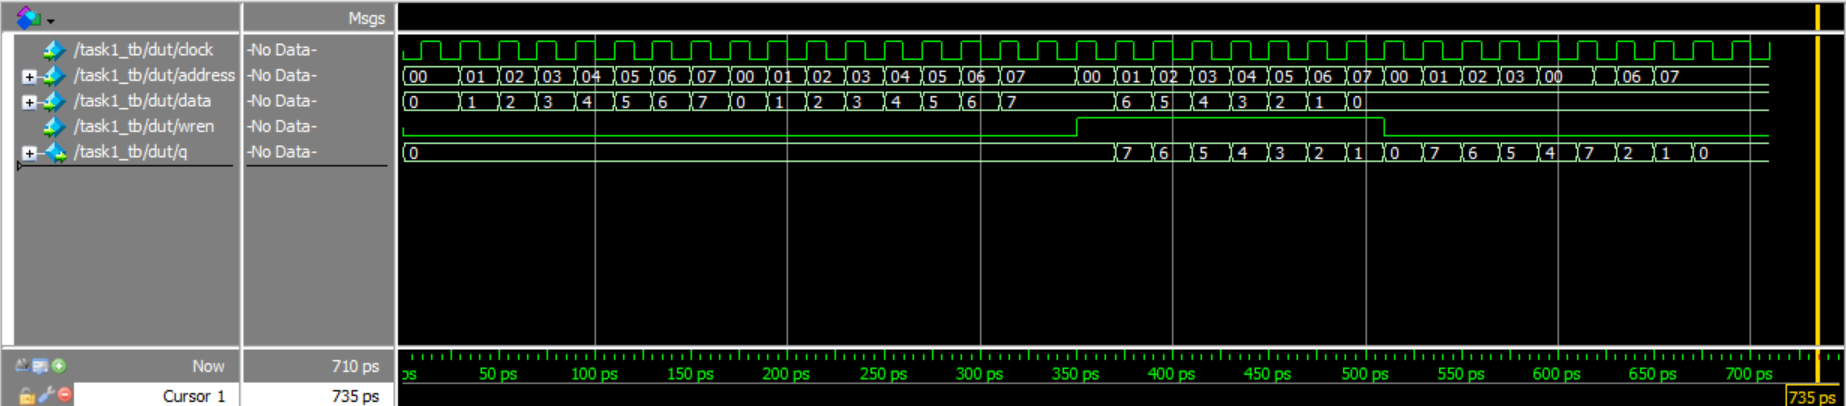
\includegraphics[scale = 0.5]{Images/task 1 testbench.png}
            \end{center}
            This testbench demonstrates the expected behavior of the ram module. It shows that when the ram module is first instantiated, the values at the addresses are 0. It also shows that nothing is written to the memory when \texttt{wren} is not on. It then shows data being written to the memory. Finally, it shows the data being read is the same data that was written.

        \subsection{Task \#2}
            The test bench for the task \#2 module can be seen below. \\

            \begin{center}
                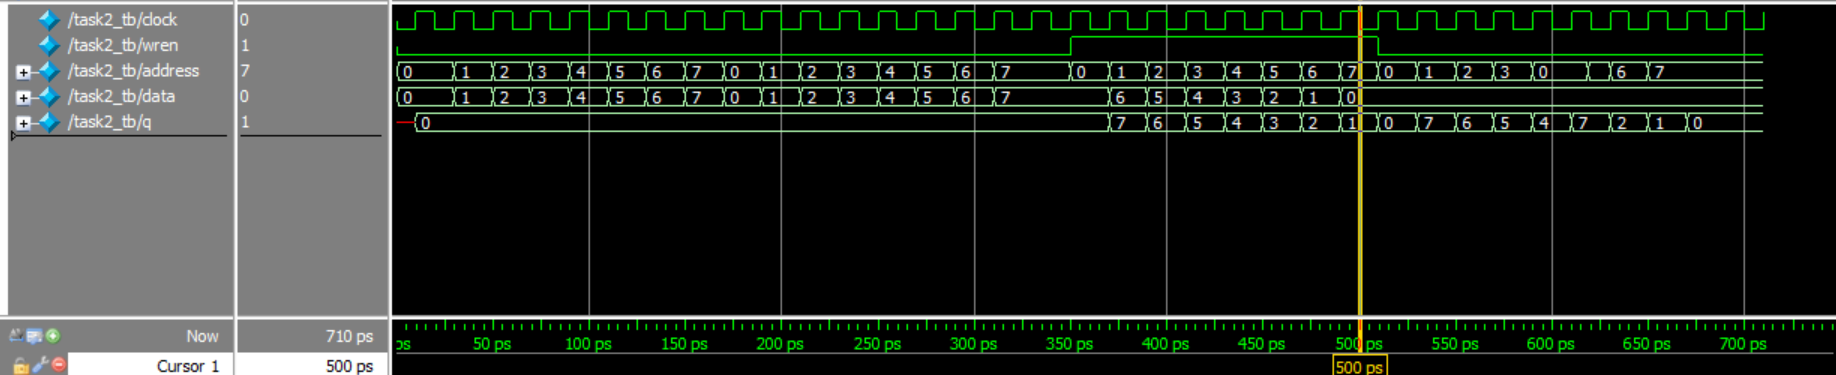
\includegraphics[scale = 0.5]{Images/task 2 testbench.png}
            \end{center}

        \newpage

        \subsection{DE1\_SoC Task \#2}
            The test bench for the DE1\_SoC module of task \#2 can be seen below. \\

            \begin{center}
                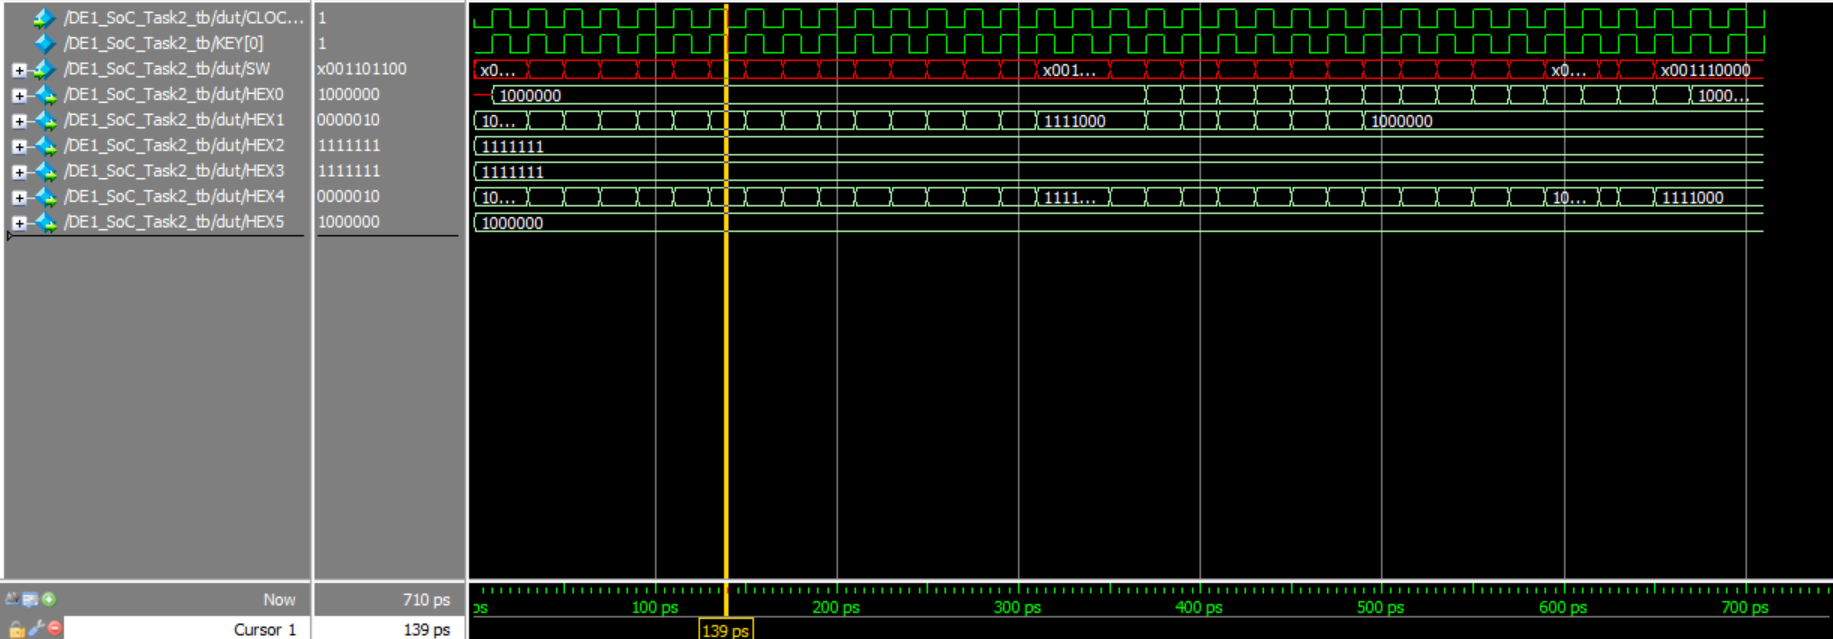
\includegraphics[scale = 0.5]{Images/task 2 DE1 testbench.png}
            \end{center}

            The inputs for this system were SW3-SW1 to specify dataIn, SW8-SW4 to specify address, and SW0 for write. The output of the system was to the HEX displays, HEX5-HEX4 for address, HEX1 for dataIn, and HEX0 for dataOut. The hex displays were controlled using a seg7 module. This testbench demonstrates that all the modules are connected correctly. The hex displays update correctly when the switches change and when data is written or read.
        
        \subsection{DE1\_SoC Task \#3}
            The test bench for the DE1\_SoC module of task \#3 can be seen below.

            \begin{center}
                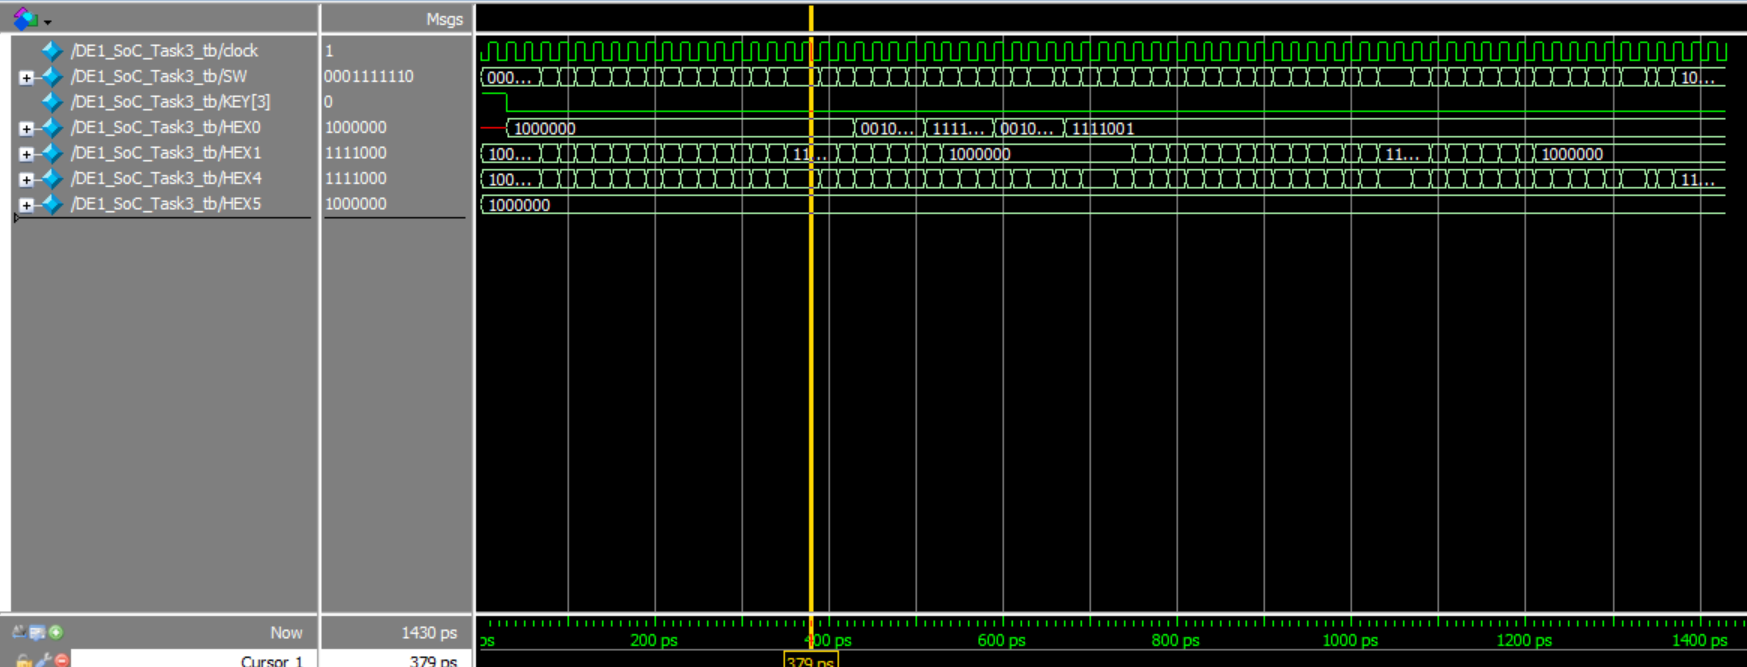
\includegraphics[scale = 0.5]{Images/task 3 DE1 testbench.png}
            \end{center}

            The inputs for this system were SW3-SW1 to specify writeData, SW8-SW4 to specify write address, and SW9 to switch from task \#2 RAM to task \#3 RAM or vice versa. The output of the system was to the HEX displays, HEX5-HEX4 for write address, HEX1 for writeData, HEX3-HEX2 for the read address, and HEX0 for read output. The hex displays again were controlled using a seg7 module. 

        \subsection{Flow Summary}
            \begin{center}
                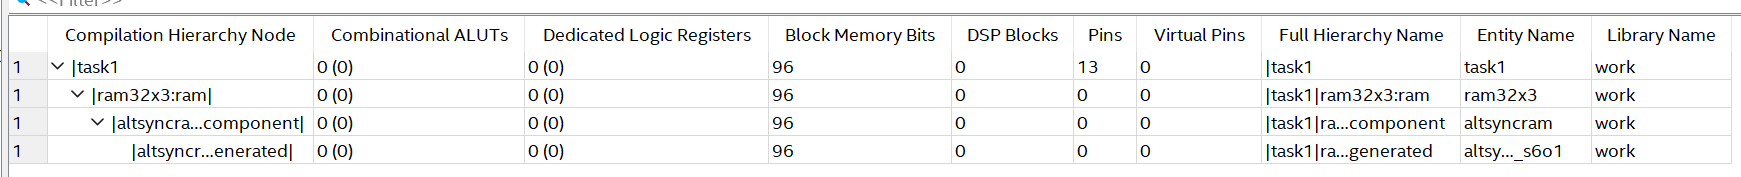
\includegraphics[scale = 0.5]{Images/task1 resouces.png}
            \end{center}

            \begin{center}
                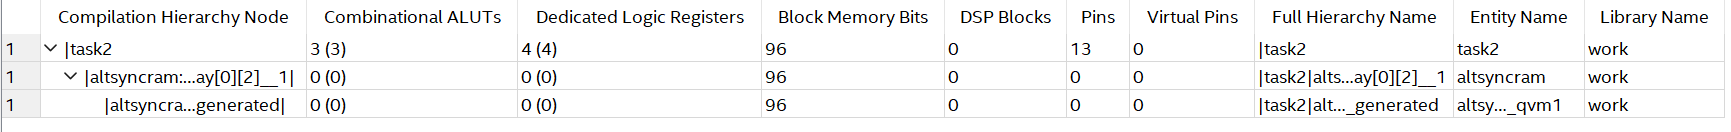
\includegraphics[scale = 0.5]{Images/task2 resouces.png}
            \end{center}

            \begin{center}
                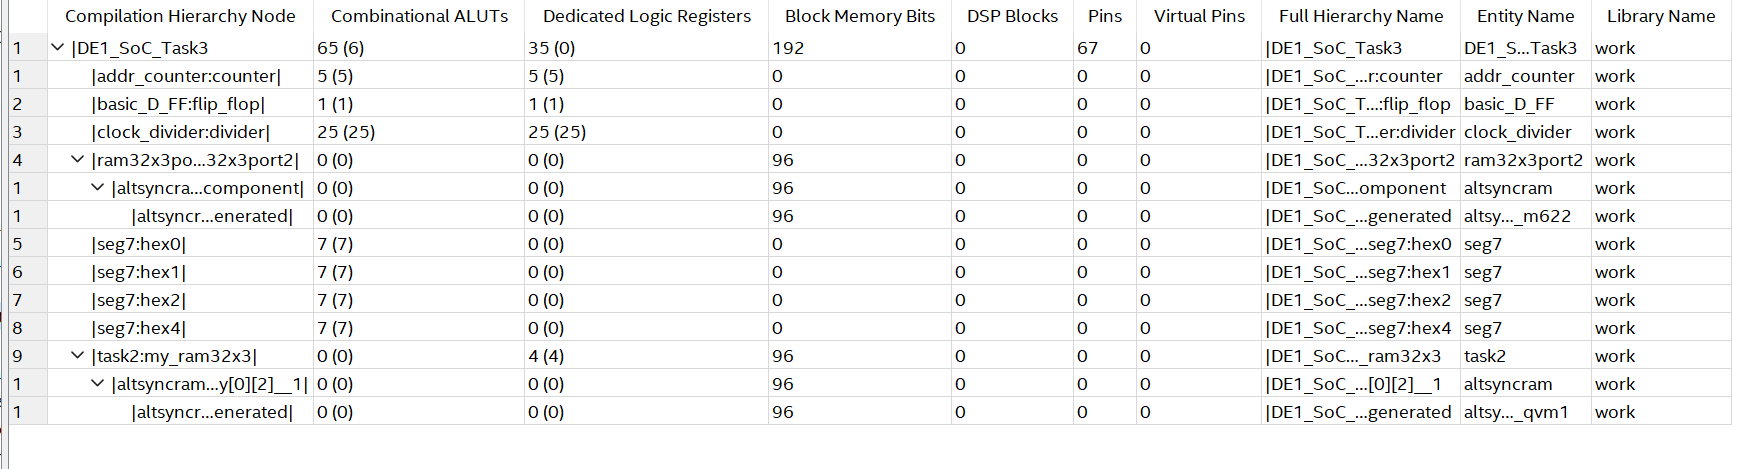
\includegraphics[scale = 0.5]{Images/task 3 resoucres.png}
            \end{center}

    \section{Experience Report}
        This lab took approximately 8 hours, broken down as follows:
        \begin{description}
            \item[Reading:] 45 minutes
            \item[Design:] 30 minutes
            \item[Coding:] 6 hours
            \item[Testing:] 1 hours
        \end{description}   
        
\end{document}
